Database gestisce l'utilizzo del database tramite le classi DatabaseManager e derivate. La suddivisione rispecchia la rappresentazione dei dati all'interno della base di dati. In particolare:
\begin{itemize}
	\item \texttt{DatabaseExerciseManager}: permette le operazioni CRUD$^{*}$ e di ricerca degli esercizi;
	\item \texttt{DatabaseClassManager}: permette le operazioni CRUD e di ricerca delle classi;
	\item \texttt{DatabaseUserManager}: permette le operazioni CRUD e di ricerca degli User.
\end{itemize}
Questa gerarchia di classi agevola, in caso di ristrutturazione dell'applicazione, la sostituzione della base di dati dell'applicazione, semplicemente cambiando il riferimento al database. In questo caso, sarà necessario modificare il riferimento della classe al database. Tale modifica sarà però circoscritta a questa gerarchia di classi senza alcuna necessità di modificare le altre classi dell'applicazione.
\begin{figure}[h]
	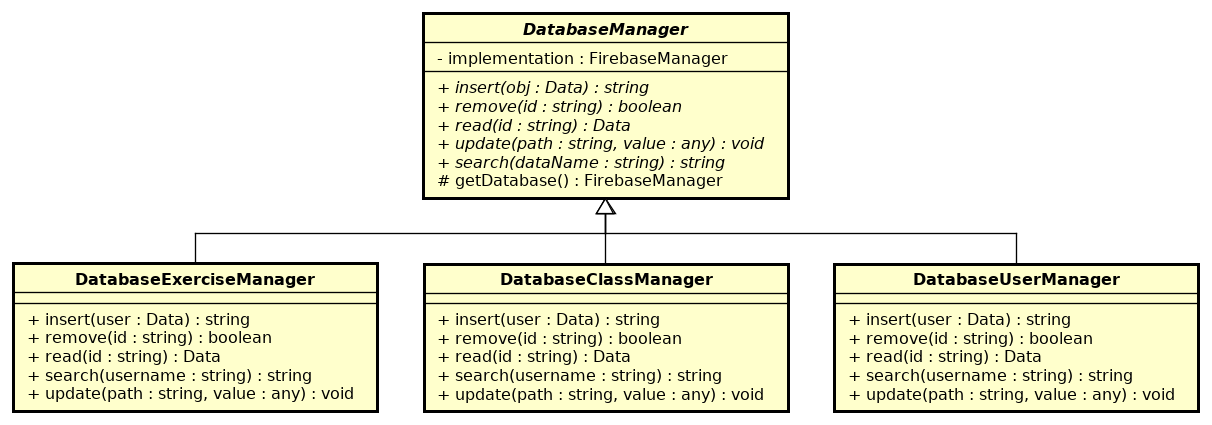
\includegraphics[scale=0.5]{images/DatabaseManager.png}
	\caption{Diagramma delle classi del package Database}
\end{figure}